%!TEX encoding = UTF-8 Unicode
%!TEX root = ../doc-omnibus.tex


\chapter{Les registres de contrôle}

%La déclaration d'un registre de contrôle obéit à une syntaxe particulière, ne serait-ce que parce que son adresse absolue doit y être spécifiée. Pour de nombreux registres, un bit ou un groupe de bits ont une signification particulière, et obtenir la valeur d'un champ ou modifier sa valeur est une opération courante.

%À titre d'exemple, nous allons nous intéresser au registre \texttt{ICSR} du processeur ARMv7-M. Le \emph{manuel de référence de l'architecture ARMv7-M}\footnote{\url{http://infocenter.arm.com/help/index.jsp?topic=/com.arm.doc.ddi0403e.b/index.html}} décrit ce registre comme indiqué à la \refFigure{}{definitionPORTxPCRn}, et indique que son adresse est \texttt{0xE000ED04}.

Dans ce chapitre, nous allons décrire~:
\begin{itemize}
  \item comment déclarer un registre de contrôle, comment lui affecter une valeur, et le lire (\refSectionPage{simpleDeclarationRegistre})~;
  \item comment déclarer les champs d'un registre de contrôle, et comment les utiliser (\refSectionPage{declarationRegistreEtChamps})~;
  \item comment déclarer plusieurs registres de contrôle ayant la même composition de champs (\refSectionPage{declarationPlusieursRegistres})~;
  \item comment déclarer et utiliser un tableau de registres de contrôle (\refSectionPage{declarationTableauRegistres})~;
  \item les attributs applicables aux registres de contrôle (\refSectionPage{attributsRegistreControle})~;
  \item les restrictions d'usage des registres de contrôle (\refSectionPage{restrictionsUsageRegistres}).
\end{itemize}

À titre d'exemple, nous allons nous intéresser aux registres \texttt{PORTx\_PCRn} du micro-contrôleur \texttt{MK20DX256VLH7} qui équipe les cartes \emph{Teensy 3.x} (\refFigure{}{definitionPORTxPCRn}). La documentation de ce micro-contrôleur indique que l'un des registres de cette famille, \texttt{PORTA\_PCR0} est à l'adresse \texttt{0x4004\_9000}.


\begin{figure}[htbp]
\centering
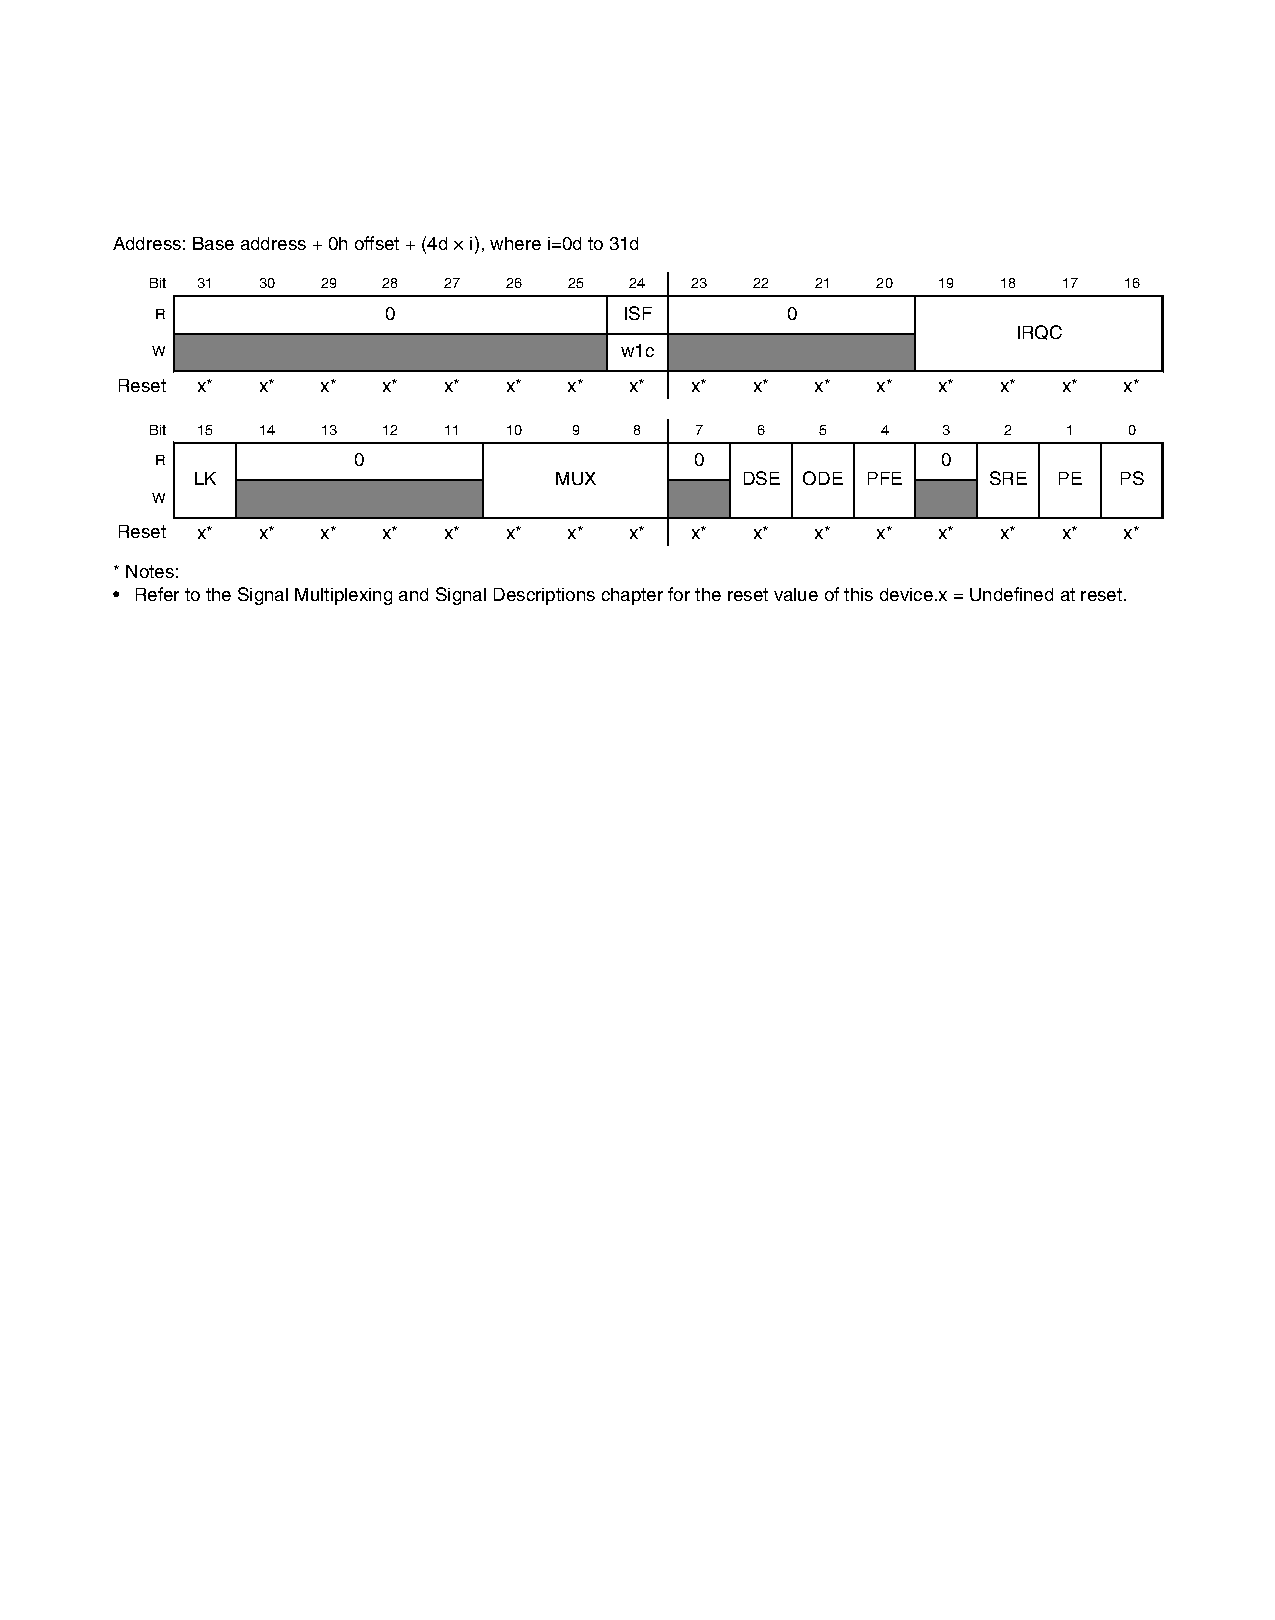
\includegraphics[width=14cm]{chapitres/PORTx_PCRn.pdf}
\caption{Registres de contrôle \texttt{PORTx\_PCRn} intégré dans le \texttt{MK20DX256VLH7}}
\labelFigure{definitionPORTxPCRn}
%\ligne
\end{figure}




\sectionLabel{Groupe de registres}{GroupeRegistre}




\sectionLabel{Simple déclaration d'un registre}{simpleDeclarationRegistre}

Pour déclarer le registre \texttt{PORTA\_PCR0} (\refFigure{}{definitionPORTxPCRn}), situé à l'adresse \texttt{0x4004\_9000}, on écrit~:

\begin{OMNIBUS}
registers ©PORTA 0x4004_9000 {
  PCR0 0x0 UInt32
}
\end{OMNIBUS}

Le type \omnibus+UInt32+ qui est mentionné signifie que les valeurs écrites et lues de ce registre sont des entiers non signés de 32 bits. Tout type entier, signé ou non signé est autorisé.

Pour lire ou écrire ce registre, on le nomme comme s'il s'agissait d'une simple variable. Par exemple, pour configurer le bit $0$ du port \texttt{A} en entrée ou en sortie logique, il faut écrire $1$ dans le champ \texttt{MUX} et zéro dans les autres champs. Comme le champ \texttt{MUX} commence au $8^e$ bit, on écrit~:

\begin{OMNIBUS}
©PORTA.PCR0 = 1 << 8
\end{OMNIBUS}

Si l'on veut que ce port soit un \emph{collecteur ouvert} si il est programmé en sortie, il faut mettre le champ \texttt{ODE} à $1$. On écrit donc~:
\begin{OMNIBUS}
©PORTA.PCR0 = (1 << 8) | (1 << 5)
\end{OMNIBUS}

Lire le contenu du registre est réalisé par une instruction d'affectation~:
\begin{OMNIBUS}
let x = ©PORTA.PCR0
\end{OMNIBUS}
Le type de la constante \omnibus+x+ est \omnibus+UInt32+, déduit du type du registre de contrôle \texttt{PORTA\_PCR0}.

Pour savoir si le bit \texttt{ODE} est activé, on réalise un masquage (l'annotation du type \omnibus+Bool+ est facultative)~:
\begin{OMNIBUS}
let ODEactivé Bool = (©PORTA.PCR0 & (1 << 5)) ≠ 0
\end{OMNIBUS}

Pour obtenir la valeur du champ \texttt{MUX}, on effectue un décalage, suivi d'un masquage~:
\begin{OMNIBUS}
let champMUX UInt32 = (©PORTA.PCR0 >> 8) & 7
\end{OMNIBUS}


Toutes ces formulations peuvent être rendues plus intelligibles en précisant la composition du registre \texttt{PORTA\_PCR0} dans sa déclaration. C'est ce qui va être réalisé dans la section suivante.








\sectionLabel{Déclaration d'un registre et de ses champs}{declarationRegistreEtChamps}

Lors de la déclaration d'un registre, il est possible de préciser la composition de ses champs entiers et booléens. Par exemple, pour le registre \texttt{PORTA\_PCR0} et en s'appuyant par sa description dans la \refFigurePage{}{definitionPORTxPCRn}~:

\begin{OMNIBUS}
registers ©PORTA {
  PCR0 0x4004_9000 UInt32 {
    7, ISF, 4, IRQC:4, LK, 4, MUX:3, 1, DSE, ODE, PFE, 1, SRE, PE, PS
  }
}
\end{OMNIBUS}

Entre accolades, trois définitions différentes peuvent apparaître~:
\begin{itemize}
\item un nombre indique le nombre de bits consécutifs inutilisés~;
\item un identificateur (par exemple \omnibus=ISF=) nomme un champ booléen~;
\item un identificateur suivi du délimteur \omnibus=:= et d'un nombre (par exemple \omnibus=IRQC:4=) nomme un champ entier constitué du nombre indiqué de bits consécutifs.
\end{itemize}

La description commence par le bit le plus significatif~: comme le type du registre est \omnibus+UInt32+ (entier non signé sur 32 bits), le premier bit nommé \texttt{ISF} porte le n°24, \texttt{IRQC} s'étend sur 4 bits à partir du n°16,~...

Cette écriture n'est autorisée que si le type nommé (ici \omnibus+UInt32+) est une type entier non signé. Les types signés (\omnibus+Int32+, ...) sont interdits. Le compilateur vérifie que la description des champs définit exactement le nombre de bits du type nommé, ici les 32 bits du type \omnibus+UInt32+.

Définir la composition des champs d'un registre permet d'utiliser des constructions qui simplifient~:
\begin{itemize}
  \item l'obtention de leur valeur (\refSubsectionPage{accesValeurChamps})~;
  \item la construction d'une valeur à affecter à un registre de contrôle (\refSubsectionPage{constructionChampEntierRegistre}).
\end{itemize}










\subsectionLabel{Accès en lecture aux champs}{accesValeurChamps}

À la \refSection{simpleDeclarationRegistre}, pour obtenir la valeur du champ \texttt{MUX} est activé, on réalisait un décalage suivi d'un masquage~:
\begin{OMNIBUS}
let champMUX UInt32 = (©PORTA.PCR0 >> 8) & 7 // 0, 1, 2, ..., 7
\end{OMNIBUS}

Plusieurs formulations nommant le champ \texttt{MUX} sont possibles.

La première renvoie la valeur du champ non décalée~:

\begin{OMNIBUS}
let résultatNonDécalé UInt32 = ©PORTA.PCR0.MUX
  // 0, 0x100, 0x200, ..., 0x700
\end{OMNIBUS}

Pour obtenir la valeur d'un champ justifiée à droite, on utilise l'accesseur \omnibus+shifted+~:
\begin{OMNIBUS}
let champMUX UInt32 = ©PORTA.PCR0.MUX.shifted // 0, 1, 2, ..., 7
\end{OMNIBUS}

L'expression \omnibus+©PORTA.PCR0.MUX.shifted+ est équivalente à \omnibus+(©PORTA.PCR0 >> 8) & 7+.


Pour le champ booléen \texttt{ODE}, on écrivait à la \refSection{simpleDeclarationRegistre}~:

\begin{OMNIBUS}
let ODEactivé Bool = (©PORTA.PCR0 & (1 << 5)) ≠ 0
\end{OMNIBUS}

On peut maintenant écrire (noter que le type du résultat est \omnibus=UInt32=)~:
\begin{OMNIBUS}
let champODEnonDécalé UInt32 = ©PORTA.PCR0.ODE // 0 ou 2**5
\end{OMNIBUS}

De même, on peut obtenir la valeur justifiée à droite (noter que le type du résultat est toujours \omnibus=UInt32=)~:
\begin{OMNIBUS}
let champODEdécalé UInt32 = ©PORTA.PCR0.ODE.shifted // 0 ou 1
\end{OMNIBUS}

Pour obtenir la valeur valeur booléenne, on utilise l'accesseur \omnibus=bool= (noter que le type du résultat est maintenant \omnibus=Bool=)~:
\begin{OMNIBUS}
let ODEactivé Bool = ©PORTA.PCR0.ODE.bool // no ou yes
\end{OMNIBUS}

L'expression \omnibus+©PORTA.PCR0.ODE.bool+ est équivalente à \omnibus+(©PORTA.PCR0 & (1 << 5)) ≠ 0+.


















\subsectionLabel{Construction à partir des valeurs de champs d'un registre de contrôle}{constructionChampEntierRegistre}

La construction particulière \omnibus+$registre {champ:expression, ...}+ permet de définir facilement la valeur à affecter à un registre de contrôle. Prenons toujours l'exemple du registre \texttt{PORTA\_PCR0} dont la composition est décrite à la \refFigurePage{}{definitionPORTxPCRn}.


À la \refSection{simpleDeclarationRegistre}, pour écrire $1$ dans le champ \texttt{MUX} et zéro dans les autres champs on écrivait~:

\begin{OMNIBUS}
©PORTA.PCR0 = 1 << 8
\end{OMNIBUS}

En utilisant la notation dédiée, on écrit maintenant~:

\begin{OMNIBUS}
©PORTA.PCR0 = {©PORTA.PCR0 !MUX:1}
\end{OMNIBUS}

L'expression \omnibus+{©PORTA.PCR0 !MUX:1}+ est équivalente à \omnibus+1 << 8+.

Si l'on veut que ce port soit un \emph{collecteur ouvert} si il est programmé en sortie, il faut mettre le champ \texttt{ODE} à $1$, et on écrivait~:
\begin{OMNIBUS}
©PORTA.PCR0 = (1 << 8) | (1 << 5)
\end{OMNIBUS}

On peut maintenant écrire~:

\begin{OMNIBUS}
©PORTA.PCR0 = {©PORTA.PCR0 !MUX:1 !ODE:1}
\end{OMNIBUS}


\subsection{Vérifications sémantiques}

Examinons maintenant les conditions de validité de l'\omnibus=expression= dans la construction (décrite à la \refSubsectionPage{constructionChampEntierRegistre}) \omnibus+{©group.registre !champ:expression, ...}+.

{\bf Expression entière statique.} Le compilateur vérifie qu'elle est comprise entre $0$ et $2^n-1$, $n$ étant le nombre de bits du champ~: par exemple, pour le champ \texttt{MUX} de $3$ bits, une valeur entre $0$ et $7$. Ainsi~:

\begin{OMNIBUS}
©PORTA.PCR0 = {©PORTA.PCR0 !MUX:1-2} // Erreur de compilation, exp. < 0
©PORTA.PCR0 = {©PORTA.PCR0 !MUX:8} // Erreur de compilation, exp. > 7
\end{OMNIBUS}

{\bf Expression entière non statique signée.} Le compilateur considère que c'est une erreur~: uniquement une expression entière non statique non signée est acceptable.


{\bf Expression entière non statique non signée.} Il y a plusieurs sous cas à examiner.

Si l'\omnibus=expression= est d'un type entier non signé dont le nombre de bits est inférieur ou égal au nombre de bits du champ, alors toute valeur de l'\omnibus+expression+ est acceptable~: le code engendré se borne à faire le décalage à gauche de la valeur de l'\omnibus+expression+.

Par exemple, le champ \texttt{MUX} s'étendant sur $3$ bits, une expression de type \omnibus=UInt3=, \omnibus=UInt2= ou \omnibus=UInt1= est toujours acceptée~:

\begin{OMNIBUS}
let x UInt2 = 1
©PORTA.PCR0 = {©PORTA.PCR0 !MUX:x} // Ok
\end{OMNIBUS}

Dans le cas contraire, c'est-à-dire si l'\omnibus=expression= est d'un type entier non signé dont le nombre de bits est strictement supérieur au nombre de bits du champ, une vérification de la valeur à l'exécution est effectuée~: si la valeur de l'\omnibus+expression+ est trop grande, la panique (code~: voir \refTableauPage{tableauCodePanique}) est déclenchée. Si la génération de code panique n'est pas activée, le débordement est silencieusement ignoré. Par exemple~:

\begin{OMNIBUS}
let x UInt8 = ...
©PORTA.PCR0 = {©PORTA.PCR0 !MUX:x} // Vérification à l'exécution
\end{OMNIBUS}

Si le code ci-dessus apparaît dans une routine où la génération de panique est interdite (par exemple, dans une routine \omnibus=boot=), alors il déclenche une erreur de compilation. Il faut ajouter une troncature explicite pour le code soit accepté~:

\begin{OMNIBUS}
let x UInt8 = ...
©PORTA.PCR0 = {©PORTA.PCR0 !MUX:truncate UInt3 (x)}
\end{OMNIBUS}

Ce code n'effectue aucune vérification à l'exécution.
















\sectionLabel{Déclaration de plusieurs registres}{declarationPlusieursRegistres}

Il est possible de regrouper les déclarations de registres partageant la même décomposition de leur champs. Par exemple, pour les registres \texttt{PORT$n$\_PCR$m$} du \texttt{mk20dx256} (seule la déclaration de deux premiers registres est montrée)~:

\begin{OMNIBUS}
registers ©PORTA {
  PCR0 0x4004_9000
  PCR1 0x4004_9004
  UInt32 {
    7, ISF, 4, IRQC:4, LK, 4, MUX:3, 1, DSE, ODE, PFE, 1, SRE, PE, PS
  }
}
\end{OMNIBUS}











\sectionLabel{Déclaration d'un tableau de registres}{declarationTableauRegistres}

Le micro-contrôleur \texttt{LPC2294} de NXP possède 4 modules CAN.

\fbox{\begin{minipage}{1.0\textwidth}
  La documentation du \texttt{LPC2294} numérote ces modules de $1$ à $4$. Dans ce document, ils sont numérotés de $0$ à $3$, ce qui s'avère beaucoup plus pratique à l'usage.
\end{minipage}}

Les registres de ces modules sont aux adresses~:

\texttt{0xE004\_4000 + (canal << 14) + register\_offset}

où \texttt{canal} vaut $0$ pour le module $0$, …, $3$ pour le module 3~; \texttt{register\_offset} est une valeur propre à chaque type de registre. Par exemple, pour les registres \texttt{CANCMR}, l'offset est égal à 4. Les quatre registres \texttt{CANCMR} sont donc aux adresses~:

\texttt{CANCMR0} : \texttt{0xE004\_4000 + (0 << 14) + 4 = 0xE004\_4004}

\texttt{CANCMR1} : \texttt{0xE004\_4000 + (1 << 14) + 4 = 0xE004\_8004}

\texttt{CANCMR2} : \texttt{0xE004\_4000 + (2 << 14) + 4 = 0xE004\_C004}

\texttt{CANCMR3} : \texttt{0xE004\_4000 + (3 << 14) + 4 = 0xE005\_0004}

Il est possible de déclarer ces registres individuellement~:

\begin{OMNIBUS}
register
  CANCMR0 0xE004_4004
  CANCMR1 0xE004_8004
  CANCMR2 0xE004_C004
  CANCMR3 0xE005_0004
UInt32 {
  STB3, STB2, STB1, SRR, CDO, RRB, AT, TR
}
\end{OMNIBUS}

Mais on n'a pas de solution simple pour sélectionner un de ces registres en fonction du numéro de module. Si on veut écrire une valeur \omnibus=v= dans le registre désigné par la variable \omnibus=n= (dont la valeur est comprise entre $0$ et $3$), il faut écrire~:

\begin{OMNIBUS}
if n == 0 {
  CANCMR0 = v
}else if n == 1 {
  CANCMR1 = v
}else if n == 2 {
  CANCMR2 = v
}else{
  CANCMR3 = v
}
\end{OMNIBUS}

On peut simplifier l'accès en déclarant les registres \texttt{CANCMR$n$} comme un tableau de registres de contrôle~:

\begin{OMNIBUS}
register
  CANCMR[4] 0xE004_4004 : 1 << 14
UInt8 {
  STB3, STB2, STB1, SRR, CDO, RRB, AT, TR
}
\end{OMNIBUS}

D'une manière générale, la déclaration d'un tableau de registres de contrôle est de la forme~:
\begin{OMNIBUS}
nom_registre [taille] adresse_base~: multiplicateur
$type { ... }
\end{OMNIBUS}

La \omnibus=taille= doit toujours être égale à une puissance de $2$. L'adresse du registre d'indice $i$ est égale à \texttt{adresse\_base + $i$ * multiplicateur}. Ici~:

Adresse de \texttt{CANCMR[0]} : \texttt{0xE004\_4004 + 0 * (1 << 14) = 0xE004\_4004}

Adresse de \texttt{CANCMR[1]} : \texttt{0xE004\_4004 + 1 * (1 << 14) = 0xE004\_8004}

Adresse de \texttt{CANCMR[2]} : \texttt{0xE004\_4004 + 2 * (1 << 14) = 0xE004\_C004}

Adresse de \texttt{CANCMR[3]} : \texttt{0xE004\_4004 + 3 * (1 << 14) = 0xE005\_0004}

Si vous voulez confirmer le calcul des adresses des registres de contrôle, utilisez l'option de la ligne de commande \OPTION{-{}-control-register-map} (\refSectionPage{optionsDebogage}) qui affiche le détail de la définition des registres de contrôle dans un fichier HTML.

L'accès aux registres de contrôle s'effectue alors en utilisant la notation \omnibus=[...]= habituelle de l'accès à un élément de tableau. Par exemple, en reprenant l'exemple précédent, écrire une valeur \omnibus=v= dans le registre désigné par la variable \omnibus=n= (dont la valeur est comprise entre $0$ et $3$) s'exprime simplement par~:

\begin{OMNIBUS}
CANCMR[n] = v
\end{OMNIBUS}

L'indice d'un tableau de registre peut-être une expression entière statique, ou une expression dynamique signée ou non signée. Les vérifications à la compilation et à l'exécution sont les même que pour l'accès à un élément de tableau (voir la \refSectionPage{AccesElementTableau}).

En particulier, si l'indice est une expression de type non signée dont la valeur maximum est strictement inférieure à la taille du tableau, aucune vérification n'est faite à l'exécution, puisque l'indice sera toujours valide~:

\begin{OMNIBUS}
let n UInt2 = ...
CANCMR[n] = v // Aucune vérification, indice toujours valide
\end{OMNIBUS}








\sectionLabel{Attributs d'un registre de contrôle}{attributsRegistreControle}

\subsectionLabel{Attribut \texttt{@ro}}{attributRo}\index{"@ro}
La déclaration d'un registre accepte l'attribut \omnibus+@ro+, qui signifie qu'il est en lecture seule. Par exemple~:
\begin{OMNIBUS}
registers {
   CALIB @ro 0xE000_E01C UInt32
}
\end{OMNIBUS}

Toute tentative de faire figurer ce registre dans une construction qui provoque une écriture de celui-ci entraîne l'apparition d'une erreur de compilation.






\subsectionLabel{Attribut \texttt{@user}}{attributUser}\index{"@user}
La déclaration d'un registre accepte l'attribut \omnibus+@user+, qui signifie qu'il est accessible en mode \omnibus!user!. Par défaut, un registre de contrôle n'est pas accessible en mode  \omnibus!user!. Par exemple~:
\begin{OMNIBUS}
registers GPIOE {
  PSOR @user 0x400F_F104 UInt32
}
\end{OMNIBUS}

Évidemment, il faut que le matériel accepte effectivement que le registre soit accessible quand le processeur en mode \emph{utilisateur}.









\sectionLabel{Restrictions d'usage des registres}{restrictionsUsageRegistres}\index{Parametre effectif@Paramètre effectif!Registre}

Un registre ne peut pas~:
\begin{itemize}
  \item apparaître comme paramètre effectif en entrée d'une procédure~;
  \item apparaître comme paramètre effectif en sortie/entrée d'une procédure.
\end{itemize}

Prenons un exemple~; la procédure \omnibus=uneProcedure= présente un argument formel en sortie, et on suppose que \texttt{REGISTRE} est un registre de type \omnibus!UInt32! :
\begin{OMNIBUS}
func user uneProcedure (!outValue UInt32) {
  outValue = 5
}
\end{OMNIBUS}



L'écriture suivante est rejetée par le compilateur (passage d'un registre comme paramètre effectif en entrée)~:
\begin{OMNIBUS}
func user autreProcedure () {
  uneProcedure (?REGISTRE) // Erreur
}
\end{OMNIBUS}

Par contre, l'écriture suivante est correcte (écriture du registre)~:
\begin{OMNIBUS}
func user autreProcedure () {
  REGISTRE = 5 // Ok
}
\end{OMNIBUS}

